\chapter{Literature Review} \label{chapter:lit-review}

\section{Architectural Description Languages} \label{sec:adl-lit-review}

Software architecture has been an active research field since the mid 1990s and one of its recurring research topics has been how to create, communicate and maintain effective architectural descriptions.  A range of techniques have been proposed over the years, but a recurrent theme is the idea of a specialised architectural description language (or "ADL").

The first ADLs appeared in the early 1990s and 10 significant languages from the first 10 years of research were the subject of a seminal literature review by Medvidovic and Taylor in January 2000 \cite{medvidovic2000-adlcomparison}.  Perhaps inspired by this work, there has been an explosion in the number of ADLs created since that time, but based on our industrial experience and reading of the research literature, there has been little indication of a corresponding increase in their use in industry.  

We are interested in how to assist architects to consider the energy properties of their systems as a first class architectural concern and this led us to ask whether we could use an ADL as the basis of any solution that we designed.   This led to our first research question namely, \emph{RQ1 - What ADLs exist and can they be used to reason about the energy properties of a system?}.  Our goal was to understand the possible applicability of existing architectural description languages to our problem and assess the degree to which the languages that have been created would be useful in industrial practice.

As part of answering this question, we undertook to identify and review the relevant research literature that has been created over twenty-five years of research in the area.  Our aim was to characterise the ADLs that have been developed and consider their possible applicability to addressing the energy properties of industrial software applications.

\subsection{Supplemental Research Questions}

As soon as we started to perform initial investigation into architectural description languages, we realised that it has become a complex and multi-faceted field.  Hence, to approach the review in a structured way, we posed a number of research questions specific to the survey, in order to understand the characterisics of the ADLs that have been designed, and their possible applicability to our problem:

\begin{description}
\item[ADL.RQ1] \emph{Which architectural viewpoints does each ADL support?}  It has been long understood that an architecture contains many structures, not just one.  This challenge is addressed by structuring an architectural description into views defined by viewpoints \cite{iso-42010}. Surveying the set of viewpoints supported by an ADL allows us to understand which architectural structures it can represent.

\item[ADL.RQ2] \emph{Does the ADL provide structuring mechanisms for large architectural descriptions?}  Many academic tools and methods are only tested using small examples whereas industrial systems are often orders of magnitude larger.  Our focus on the industrial application of ADLs meant that we wanted to understand which ADLs included features for structuring large architectural descriptions.

\item[ADL.RQ3] \emph{Does the ADL support the analysis of an architecture?}  Another possible motivation for using an ADL is the ability to perform automated analysis of a machine-readable architectural description, and this could allow the ADL to provide the basis for automated energy estimation and analysis. Hence we were interested to understand which ADLs allow this and what sort of analysis could be performed.

\item[ADL.RQ4] \emph{Can system qualities or quality requirements be captured in the ADL?}  A critical aspect of industrial software architecture work is ensuring that systems exhibit their key quality properties, so we wanted to establish what support each ADL provided to support this process.

\item[ADL.RQ5] \emph{Were prototype or production quality tools developed with the ADL?}  It is unlikely that an ADL will be seriously applied in industry unless it has robust and user-friendly tools available to support it, so we wanted to verify the level of tool support provided with each ADL.

\item[ADL.RQ6] \emph{Has the ADL been applied to non-trivial problems outside the group of people who created it? (e.g. significant research projects from outside the originating group, industrial case studies or industry standards.)}  A software architecture practitioner is likely to want some evidence of the effectiveness of an ADL before adopting it on a significant project.  Therefore, we wanted to know whether researchers had acknowledged this barrier to adoption and had addressed it through realistic case studies or use on real projects outside the originating research group.

\end{description}

It is worth noting that we do not ask if the language supports first class components because this is a prerequisite to the language being included in the study.  (Our view is that languages that do not support first class components are not architectural description languages.) 

\subsection{Research Methodology}

We identified the research literature to include in the study using an electronic literature search, augmented by manual scanning of reference lists in the papers found and our own background knowledge of the field, that led us to identify additional relevant candidate literature (that for example may not have been tagged with the keywords we expected).

We began by searching a range of electronic sources for papers that included the keywords "ADL" or "architecture description language" in their title or keywords.  The four primary sources we used were the ACM Digital Library (advanced search), Google Scholar, IEEEXplore and Microsoft Academic Search.

Predictably these queries returned many references, however it was clear from our existing knowledge of the field that these keyword-based searches were not returning all ADL related literature. 

To find further relevant literature we then performed an exhaustive search of Google Scholar, using the relevant keywords, which returned over 10,000 references which were manually scanned for relevant primary studies that we might have missed.  This list contained many false positives, but these were discarded via manual inspection. 

Having searched traditional literature review sources, we also performed manual searches of specific publication venues where ADL researchers were known to publish their findings, specifically the specialist conferences WICSA, QoSA, ECSA and ICSE.

Finally, we performed forward and backward reference checking on the primary studies that we had found. Search engines were used to find citations of the primary studies identified that could be of relevance to the review (forward reference checking). The reference lists of the primary studies were then checked for any potential relevant studies missed (backward reference checking). At this point we were left with 135 potential primary studies for the survey.

Throughout these search activities, we limited the dates of the studies that we included, to limiting our scope to literature published between January 1991 and May 2016. The start date was selected to be early enough to include all those ADLs in the original work \cite{medvidovic2000-adlcomparison} that inspired us to undertake this later comprehensive survey and as noted in \cite{malavolta2013-industryadlneeds} the concept of an ADL was not well defined before this point.  Our literature search was concluded in May 2016, which is the reason for the end date (although in fact we did not discover any additional relevant literature published between January and May 2016).

To focus our efforts on the most relevant ADLs, our initial set of primary studies was filtered further to a more manageable set using the following exclusion criteria:

\begin{description}
\item[EC1] The ADL is a minor enhancement or minor extension to an existing ADL, or the ADL is a different version of an included ADL.
\item[EC2] The ADL focuses on a single area of architectural analysis (e.g. Concurrency) rather than being a general-purpose description language.
\item[EC3] There is not enough detail in the references discovered to address the study research questions.
\item[EC4] The ADL not suitable for modelling a software intensive system at an architectural level of concern (for example a hardware design language or source code module description language).
\item[EC5] The primary study is not available in English or is a short paper (less than 3000 words), abstract, keynote, opinion, tutorial summary, panel discussion, technical report, presentation slides, compilation of work or a book chapter. Book chapters were only included if they were conference or workshop proceedings (e.g., as part of the LNCS or LNBIP series) and are available through the data sources included in our review. 
\end{description}

The result of this further selection exercise was a list of 51 ADLs to include in the survey and 84 ADLs that did not meet our inclusion criteria.  A full list of the ADLs that met our inclusion criteria are characterised in the tables in \aref{appendix:adl-list}.

\subsection{Analysis of the Results}

The first aspect of the ADLs we were interested in was the \emph{basic information} about each and specifically institution(s) who developed them, the dates when the language was first published, the application domain that they address and the breadth of the application that they have been applied to.

When considering the breadth of application of the languages, we identified five possible degrees of application of an ADL that were of interest to us, namely:
\begin{itemize}
	\item "Examples", meaning that the language has only been used to create characteristic examples of its use;
	\item "Experiments", where it has been used to model realistic problems, but only for the purpose of investigating the language;
	\item "Case Studies", meaning that it has been applied to realistic problems from outside the originating research group but by the language creators;
	\item "Research Projects", where the language has been used on other research projects by researchers other than its creators; and
	\item "Industrial Projects", meaning that the language has been used by industrial software engineering teams on real projects (rather than industrial researchers, who would be classified as research project use).
\end{itemize}

We were obviously particularly interested in how many ADLs had been applied beyond its creating research group on other research projects, or ideally on industrial projects.

The complete data set for the ADL's basic characteristics extracted from the literature can be found in \tref{table:adl-basics}.

Two characteristics of the ADLs we wanted to understand were the application domains that they targeted and the degree to which they had been applied.

\begin{figure}
\centering
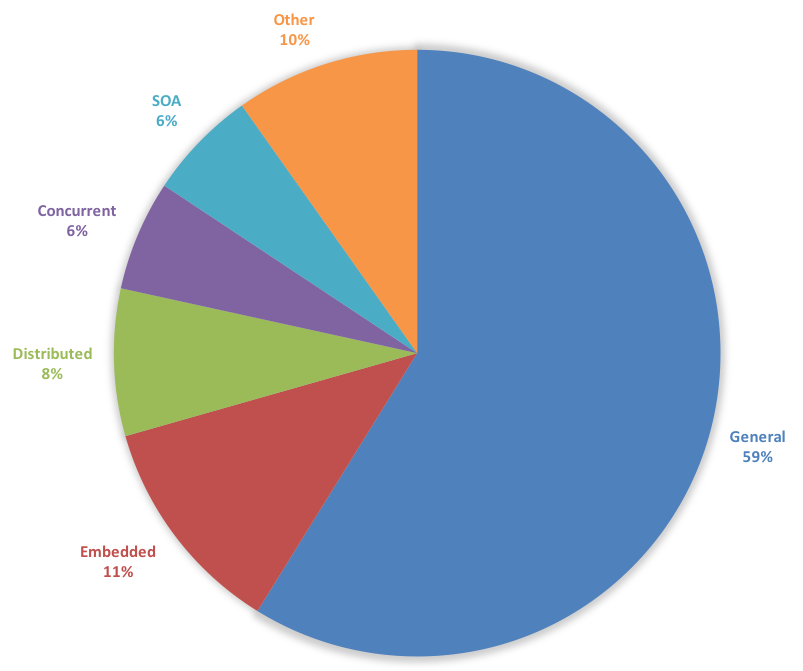
\includegraphics[width=0.6\textwidth]{Figures/litreview-adl-domains}
\caption{ADL Target Application Domain}
\label{figure:litreview-adl-domains}
\end{figure}

The analysis of the intended application domain of the languages can be found in \fref{figure:litreview-adl-domains}.  Interestingly very few of the languages were created for a specific business domain (e.g. financial analysis or industrial control systems) as over half the ADLs in the study do not explicitly target any business or technical application domain but are for general use.  There are a smaller number of ADLs specialised for embedded systems, distributed systems, highly concurrent systems and SOA, along with a number of individual ADLs for niche domains such as cyber-physical systems.

\begin{figure}
\centering
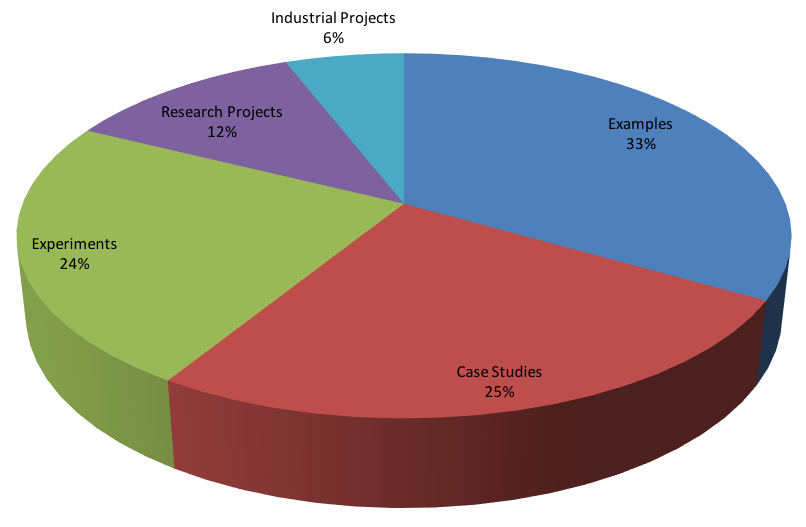
\includegraphics[width=0.6\textwidth]{Figures/litreview-adl-validation}
\caption{ADL Breadth of Application}
\label{figure:litreview-adl-validation}
\end{figure}

The analysis of the breadth of application of the languages can be found in \fref{figure:litreview-adl-validation}.  Unfortunately, as can be seen, less than 20\% of ADLs have been used beyond the case study level to perform significant research or industrial projects, suggesting a low degree of validation and practical experience with most of the languages.

The second area of interest to us were the \emph{architectural concepts} available in the different languages, to see if common industrial architectural concepts where in the languages or would need to be added.

The characteristics we analysed the ADLs for were the viewpoints that the ADL directly supports, the architectural concepts that they provide, whether they provide the ability to define behavioural semantics, whether they provide first class connectors and whether they provide first class architectural configuration constructs.  We chose to focus on these architectural concepts because of their wide use in the existing research literature and their general familiarity as concepts in industrial practice.

We were particularly interested in which viewpoints each ADL could support, as industrial architectural description nearly always needs a number of views to describe it, and the views supported provide a good insight into what the language can be used for.

None of the ADLs discuss a specific set of viewpoints that they define, so we analysed whether they provided effective support for the 6 viewpoints from \cite{rozanski2011-ssa2e} (which are Functional, Concurrency, Information, Development, Deployment and Operational).  We class a language has having first class connectors if the connector is defined separately to components and so is potentially reusable.  Similarly we consider architectural configuration to be a first class concept if it is described separately to the architectural elements and defines how they are combined, rather than being defined implicitly as part of the definition of the elements.

The complete data set for the architectural concepts available in each of the ADLs can be found in \tref{table:adl-concepts}.

The analysis of which viewpoints are supported by the different ADLs is presented in \fref{figure:litreview-adl-viewpoints}.

\begin{figure}
\centering
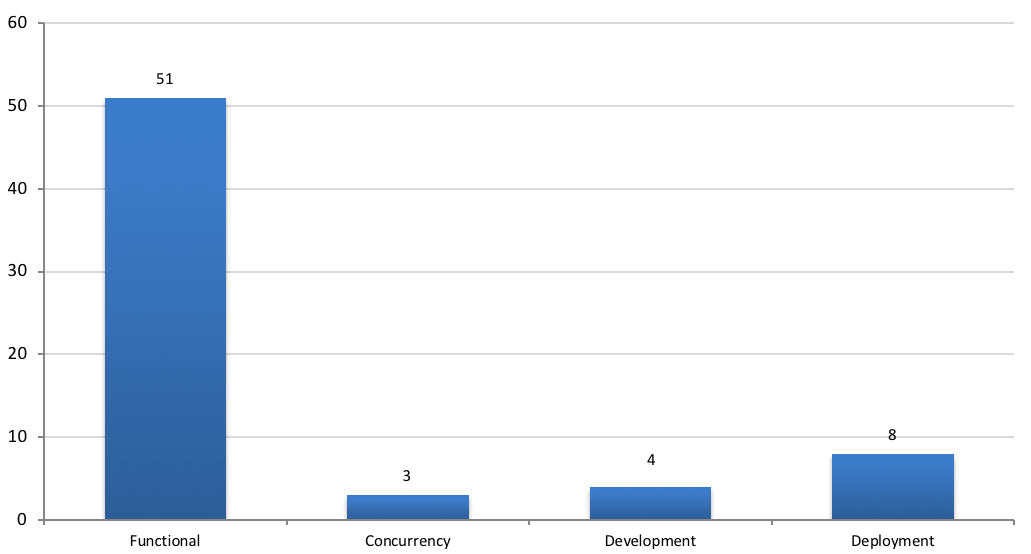
\includegraphics[width=0.75\textwidth]{Figures/litreview-adl-viewpoints}
\caption{Viewpoints Supported by ADLs}
\label{figure:litreview-adl-viewpoints}
\end{figure}

What is immediately evident from this analysis is that most ADLs only focus on the functional view of a system (i.e. its functional components and connectors and their organisation).  While clearly a key part of a system's architecture, most architects actually spend a lot of their effort working on other parts of an architecture (such as the deployment of the system).  So most of these ADLs are at best a partial solution to the problem of industrial architectural description.

\begin{figure}
\centering
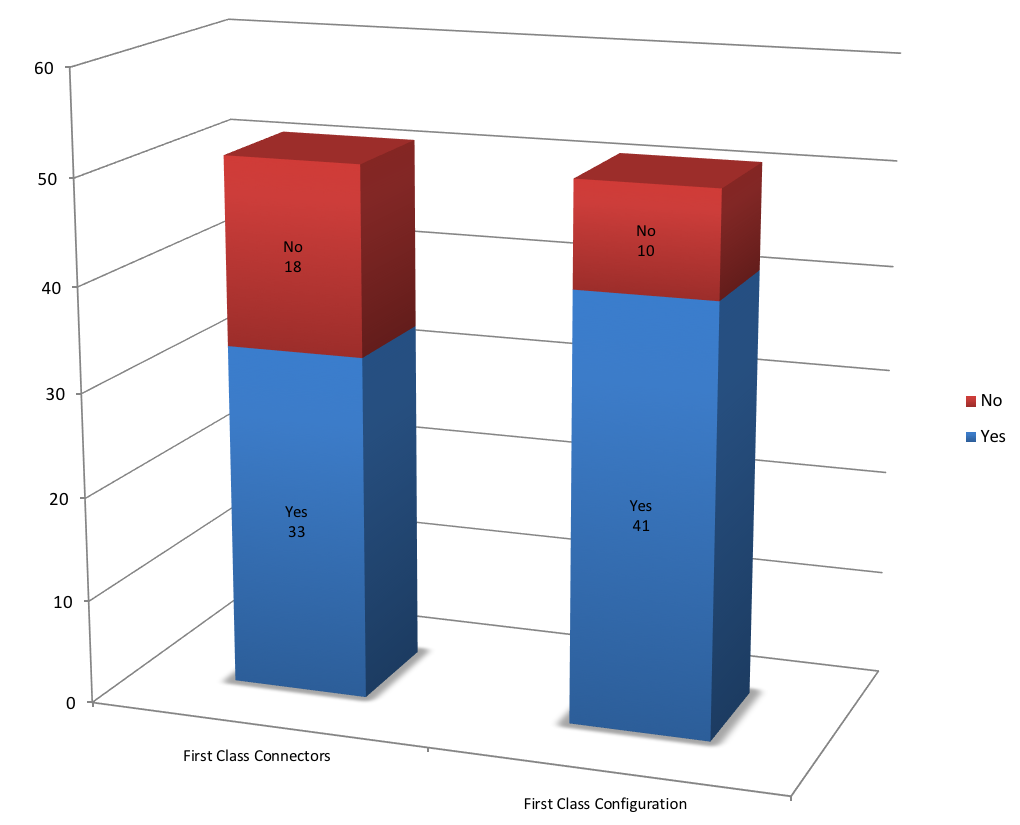
\includegraphics[width=0.75\textwidth]{Figures/litreview-adl-candc}
\caption{Connector and Configuration Support}
\label{figure:litreview-adl-candc}
\end{figure}

The analysis of the number of ADLs that provide support for first class connectors and architectural configuration as a first class concept is shown in \fref{figure:litreview-adl-candc}.

This analysis reveals a very positive result, as the clear majority of ADLs in the study provide some form of first class configuration, while less, but still nearly two thirds, provide support for first class connectors, which are both possible motivating factors for architects to use ADLs as existing informal and semi-formal notations tend not to support these concepts directly.

The third area of interest to us were the \emph{language mechanisms} available in the different languages, to assess the languages to see whether they could address common challenges (such as structuring and evolution) for large industrial architectural descriptions.

The attributes of the language that we analysed the literature for were as follows:
\begin{description} 
	\item[Structuring] - what mechanisms are available for structuring a large architectural description?
	\item[Evolution] - what mechanisms are provided to allow an architect to evolve an architectural description?  (Such as the ability to describe architectural variations, the ability to version all or parts of the description or support for dynamic architectures).
	\item[Qualities] - how provided or required architectural properties can be captured in the architectural description (e.g. properties, attributes, related models etc.).
	\item[Syntax] - what concrete syntaxes are available to capture architectural descriptions in the language?
	\item[Analysis] - how analysis of an architectural description could be supported using the language and any supporting technologies associated with it.
	\item[Tools] - what maturity are the tools that have been created to support the language? This can be "none", "prototype" (meaning an initial tool implementation applied to small problems), "research" (meaning a fully implemented tool applied to realistic problems by researchers), and "commercial" meaning that one or more tools have been implemented and used in an industrial context by people other than the tool's creators.
\end{description}

\begin{figure}
\centering
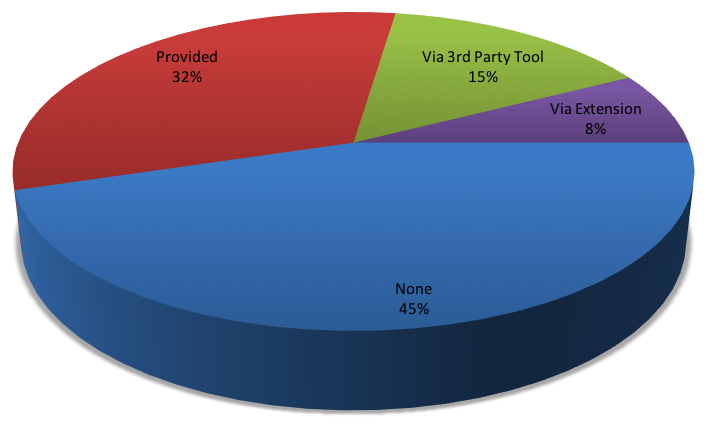
\includegraphics[width=0.6\textwidth]{Figures/litreview-adl-analysis}
\caption{ADL Support for Architectural Analysis}
\label{figure:litreview-adl-analysis}
\end{figure}

A common justification for using ADLs is the ability to perform automated analysis on the architectural description once it is represented using an ADL.  Therefore, we were interested to understand how many ADLs provided some sort of direct support for analysis of architectural descriptions.  

When we performed this analysis, we found that it was quite difficult because the analysis capabilities depend on support tools as much as the language and different ADLs provide quite different types of analysis capabilities.  To allow us to answer the question, we have defined four types of analysis capability:
\begin{description}
	\item [Provided] - where the ADL has specific support in the language to capture the data necessary to allow an automated tool to use it for analysis and explicit consideration has been given to making this possible.
	\item[Via Extension] - where the ADL has been designed such that its extension mechanisms could be used directly to support automated analysis via a tool.
	\item[Via 3rd Party Tool] - which means that the ADL provides some generic facilities that could allow a 3rd party tool to perform automated analysis, but where no explicit support for it is provided.
	\item[None] - where the language does not appear to be amenable to automated analysis.
\end{description}

This analysis is presented in \fref{figure:litreview-adl-analysis}.  As can be seen, less than half of the languages appear to provide realistic possibilities for automated analysis (and of course of those that do, many do not have working tools available for them).  We conclude therefore that automated analysis is only of interest in a subset of research groups working on ADLs.  A concern that we have with this situation is that an important motivator for adopting ADLs does not appear to be addressed in many of the ADLs that have been created.

\begin{figure}
\centering
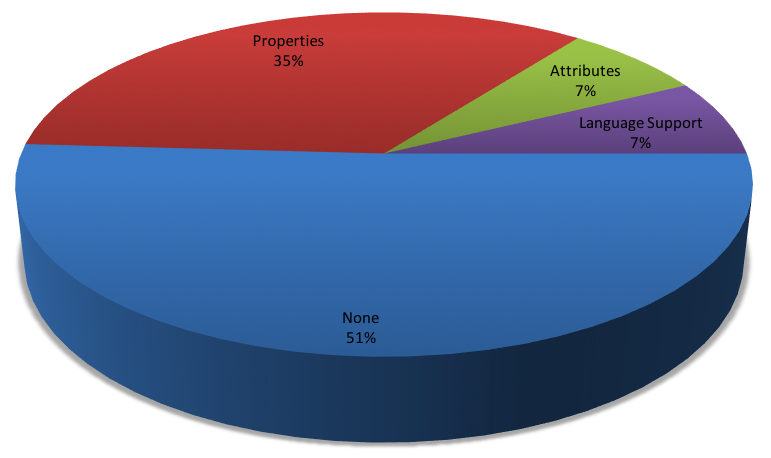
\includegraphics[width=0.6\textwidth]{Figures/litreview-adl-qualities}
\caption{ADL Support for Capturing System Qualities}
\label{figure:litreview-adl-qualities}
\end{figure}

A key goal of software architecture is to ensure that a system achieves the set of quality properties required for it to be successful.  This lead us to expect that ADLs would provide strong support for quality properties and we were interested in the types of mechanism used to represent them.  Having read the literature, we discovered that there were three broad levels of support for capturing quality properties in an architectural description:
\begin{description}
	\item[Properties] - where a generalised mechanism of (possibly typed) name/value pairs was available in the language and could be used to capture non-functional requirements and qualities but is not specifically provided for that purpose.
	\item[Attributes] - where specific pre-defined attributes relating to specific qualities (such as "transactions per second" for performance or "max connections" for scalability) can be captured within the language framework.
	\item[Language Support] - the case where languages provide a specific mechanism within the language for capturing quality requirements and capabilities (such as capturing security mechanisms and goals as first class language elements or providing a general purpose QoS or quality requirements sublanguage).
\end{description}

\fref{figure:litreview-adl-qualities} presents our analysis of this aspect of the capability of the ADLs.  It shows clearly that half of the languages provide no support for capturing system qualities, but that about a third (35\%) do have a generic properties mechanism which could be used to capture quality related information.  A much smaller number provide the ability to capture specific attributes (7\%) or have quality property features in their language (8\%).

\begin{figure}
\centering
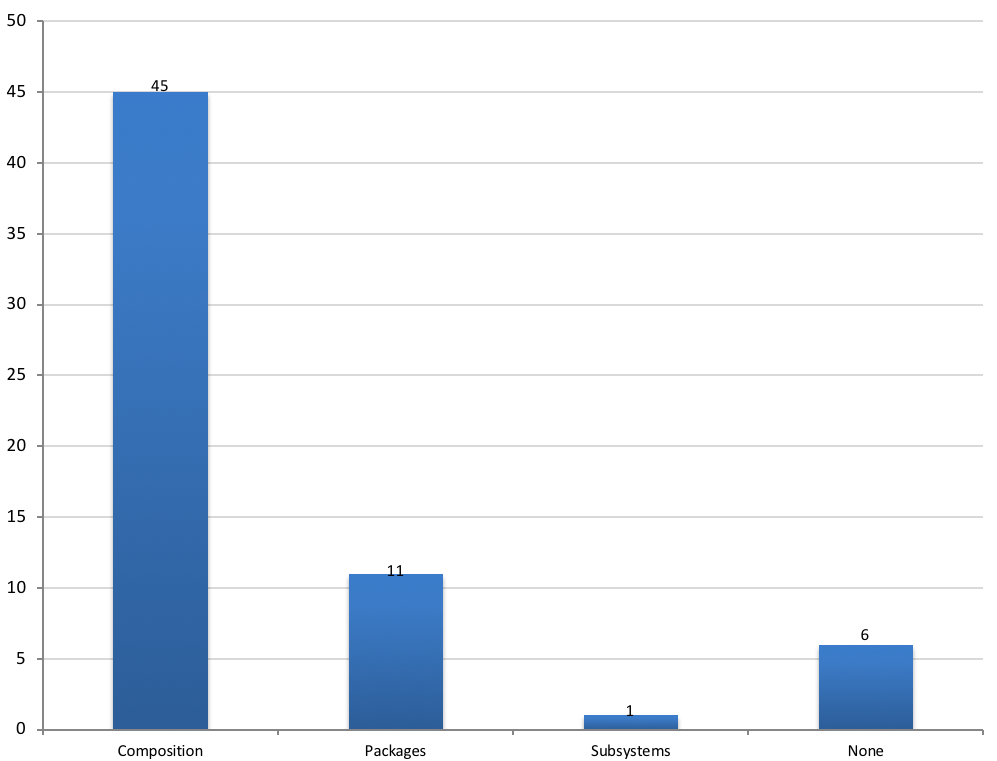
\includegraphics[width=0.75\textwidth]{Figures/litreview-adl-structuring}
\caption{Support for Structuring Architectural Descriptions}
\label{figure:litreview-adl-structuring}
\end{figure}

Many industrial systems are large, much larger than any case study or prototype experiment in the research domain.  A typical industrial system today can contain 500,000 to 1mm lines of code and dozens to hundreds of architectural elements.  Such systems cannot be described using languages that do not have effective structuring mechanisms to allow a system description to be broken down into smaller discrete parts.  This led us to investigate the mechanisms that each of the ADLs in the study provided for structuring the architectural description.  This analysis is shown in \fref{figure:litreview-adl-structuring}.

While a few of the ADLs (about 12\%) don't provide a structuring mechanism, most do, with nearly all of them offering \emph{composition} and a few offering \emph{packages} or \emph{subsystems} (in most cases in addition to composition - hence the total of values in the chart is larger than the number of ADLs in the study).
This is an interesting result, suggesting that most ADLs can be structured for large architectural descriptions, but that most of them utilise composition as the mechanism to achieve this, rather than providing a separate structuring mechanism like packages or subsystems.  This may imply restrictions in the flexibility of the structuring facilities available in those languages where only composition is available.

\begin{figure}
\centering
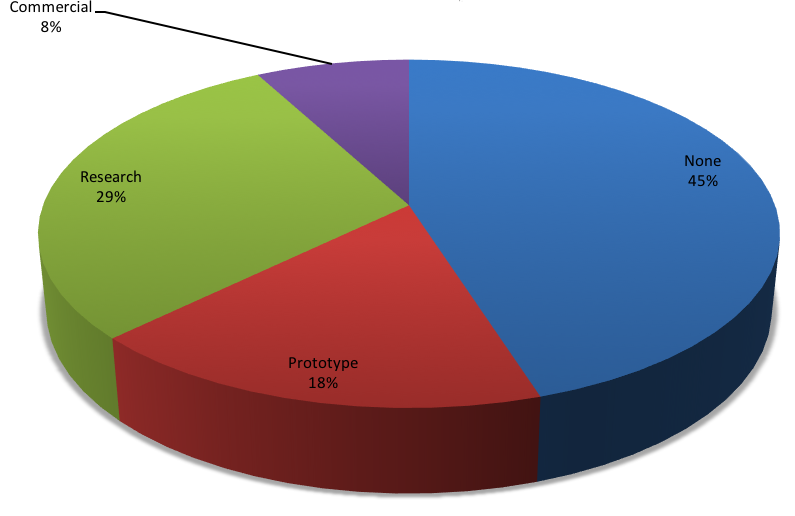
\includegraphics[width=0.6\textwidth]{Figures/litreview-adl-toolsupport}
\caption{Tool Support Available for ADLs}
\label{figure:litreview-adl-toolsupport}
\end{figure}

ADLs are often developed in conjunction with supporting tools to help architects to use them, which makes them more attractive for use on significant projects. \fref{figure:litreview-adl-toolsupport} presents our analysis of this feature of the ADLs in the study.

As can be seen, a very small percentage of the ADLs have commercially proven tools available to them, while about a third of them have tooling being used on research projects.  Nearly two thirds of the ADLs in our study provided no effective tool support.

\subsection{Conclusions}

\begin{description}
\item[ADL.RQ1] \emph{Which architectural viewpoints does each ADL support?}
All the ADLs in the study can represent functional views of the system and most of them only provide support for this view, but a small number of them allow deployment, concurrency or development views to be created too. Hence we conclude that the focus of most ADL research groups is how to represent the system's functional structure. This isn't surprising given how central a functional view is for most systems, but given the general acknowledgement of the importance of other viewpoints \cite{bachmann2011-documenting, brown2018-sad, kruchten1995-4plus1, rozanski2011-ssa2e} it does suggest that most of the existing ADLs will not be a complete solution to the problem of representing a software architecture.

\item[ADL.RQ2] \emph{Does the ADL provide structuring mechanisms for large ADs?}
Most ADLs in this study (45) provide the ability to structure a large architectural description by allowing composition of architectural elements (of course composition can also be used for other purposes, such as information hiding).   A smaller number provide specific mechanisms for structuring such as packages (11) and subsystems (1).  A few ADLs, surprisingly, do not appear to provide a structuring mechanism (6).  Some of the languages provide more than one mechanism that can be used to structure an AD (e.g. packages and composition) and this is why the numbers above sum to more than the number of ADLs in the study.\\
It is encouraging that most of the ADLs we surveyed provide at least basic facilities for structuring a large architectural description. This suggests that serious consideration has been given to the use of the ADL for realistic problems.  Those languages that don't allow structuring are presumably in an early stage of development or are not intended for industrial use.

\item[ADL.RQ3] \emph{Does the ADL support the analysis of an architecture?}
We found that about half of the ADLs (24 or 45\%) do not appear to allow a realistic option for automated analysis of architectural descriptions, which was something of a surprise to us.  Some of the languages do provide this though, with about 32\% of them providing direct support in the language, while 15\% allow this by providing mechanisms for 3rd party tools to embed information in the architectural description and 8\% allow for analysis by providing an extension mechanism that could allow analysis information to be added to an architectural description. \\
A clear motivation for capturing and maintaining an architectural description is the ability to gain useful and reliable automated analysis that can provide insight into the design that is otherwise difficult to obtain.  The fact that many ADLs being developed do not appear to provide analysis capabilities suggests that the problem of how to motivate others to use the language is often not part of the research process.

\item[ADL.RQ4] \emph{Can system qualities or quality requirements be captured in the ADL?}
Quality properties are central to the role and activities of the software architect and so we hoped for strong support for capturing qualities and quality requirements in the ADLs.  In fact, we found that more than half of the ADLs studied (28) do not appear to offer a facility to capture qualities and of those that do, most of them just provide a generic "properties" mechanism which can be used for a range of purposes including capturing qualities.  Only about 7\% of the languages provide quality property specific attributes in the language or include the ability to describe qualities as first class elements of the language.  This is a surprising situation, if the ADLs are expected to be used in an industrial setting.  Years of practical experience have taught us that achieving quality properties is a key objective of a software architect \cite{brown2018-sad, rozanski2011-ssa2e}, so we would have expected that supporting quality properties would have been an important requirement for an ADL.

\item[ADL.RQ5] \emph{Were prototype or production quality tools developed with the ADL?}
Given the importance of tool support in achieving adoption of new software technologies, we were surprised to find that 45\% of the ADLs in this survey do not appear to offer tool support that is ready for widespread transfer to industry and use.  29\% of the ADLs provide a tool that has been used for a research problem, and only 8\% of the ADLs have an associated tool that has been tested in an industrial context.\\
An important factor in applying ADLs on industrial projects is good tool support, preferably through extending tools that industry uses already.  In fact, we would go so far as to suggest that industrial adoption of any ADL without practical tool support is unlikely.

\item[ADL.RQ6] \emph{Has the ADL been applied to non-trivial problems outside the group of people who created it?}
Given the effort required to develop ADLs, we assume that most of them are intended for eventual technology transfer to industry.  Assuming so, the current degree of transfer out of the research groups is disappointing.  We found that 58\% of the ADLs have only been used by their creators, to create simple examples or experiments.  Another 26\% of the languages have only been used for case studies, again by their creators.  12\% appear to have been used for research projects, outside the creating group, while a mere 6\% of the languages have been applied in an industrial context. \\
It is our opinion that a technology can only be considered have had an impact when it is used by people other than its creators, and when considering the products of research groups, this means significant usage outside the originating research group and ideally in an industrial context.  Nearly all the ADLs we have surveyed fail this test, with less than 20\% of them having been used outside their originating group (based on the publications we could find).  It is possible that some of these ADLs have been used industrially but the case studies not published, however we feel that this is unlikely given the positive impact that publishing such case studies would have.  We believe that this finding in itself is cause for reflection within the ADL research community (as was the previous similar finding from a workshop some years ago \cite{woodshilliard2005-adlsinpractice}).
\end{description}

\section{Prioritisation of Architectural Effort}
\label{section:litreview-prioritisation}

An observation we have made from software architecture practice is that the prioritisation of an architect's activity is a complex process, with many factors being taken into account. The software architect had broad responsibilities on a project and they can be involved in almost any technical aspect of a project at some point in its lifecycle. This can make it difficult for an architect to prioritise their effort in such a way that they have the time available to prioritise quality properties like energy efficiency that are often not explicity prioritised by many of the system's stakeholders (we've observed that similar problems often occur with security, performance and scalability properties).

This situation led to our second research question \emph{RQ2 - How can architects prioritise their attention on energy efficiency?}

We do not observe role-specific heuristics or techniques in common use in industry and so were interested in whether there were approaches in the research literature which could be taught to new architects to allow us to further our goal of making it easier for software architects to address energy efficiency as an architectural concern.  

We were aware of generic time management techniques (like \cite{allen2015-gettingthingsdone} and \cite{koch1998-8020principle}) but we wanted to provide more tailored and prescriptive advice, specific to software architects, rather than more general advice of the sort found in these techniques.

We were also already aware of an entire architectural method, called Risk and Cost Driven Architecture (RCDA), designed by Eltjo Poort \cite{poort2012-rcda}, which guides software architects to focus their attention is using risks and costs.  This method transforms the architect's approach from defining finished architectural structures at the start of a project, to working throughout the project to provide a stream of decisions, using the risk and cost of open decisions to prioritise the architect's work. It can certainly help architects to focus attention on their most important concerns and might well lead architects to consider energy efficiency more often if it was widely applied.  However we know that RCDA is not very widely applied across the industry and so we were interested in whether there were simpler approaches that required less commitment to adopt.

\subsection{Research Methodology}

We identified the research literature to include in the study by searching commonly used literature catalogues as well as manually inspecting the reference lists of relevant papers and following other relevant references found.

After some experimentation we defined our search query for online catalogues to be \emph{("software architect" or "software architecture") AND ("prioritize" OR "prioritisation" OR "focus") AND ("attention" or "effort")}.  The syntax of the query had to be refined for different catalogues as they provide different search facilities, but this was a simple matter of performing multiple simpler queries against them.

We searched key online literature catalogues for papers that matched our query in in their title, abstract or keywords.  The four catalogues we used were the ACM Digital Library (advanced search), Google Scholar, IEEEXplore and Microsoft Academic Search.

The different catalogues returned different result sets for the query, with ACM Digital Library returning 11 results, IEEEXplore 12, Google Scholar nearly 80 and Microsoft Academic Search 12.

We then consolidated these results, by concatenating and removing duplicates from the ACM and IEEE results and manually scanning the results from Google Scholar to identify studies which suggested some aspect of prioritisation in their title (which resulted in 6 additional unique entries).  Finally, Microsoft Academic Search returned relatively few entries and most were obviously not relevant to our search, but 4 additional items were added manually from this source.

When we inspected the results, it became obvious that there was a significant body of literature on the subject of prioritising system quality requirements.  This is not exactly what we ask in our research question, which is more general, but we judged that such approaches might provide answers to the question, so we investigated them further.  A manual process of reference following and additional searches revealed that many of the studies in this area have little or no consideration of industrial usage or validation.  However we did find some that appeared to have potential industrial relevance and this resulted in another 20 studies which had not been returned by our search query but we believe are representative of this research area.

At this point we had a list of 46 candidate studies for consideration.

To narrow the list to the most relevant for our needs, we identified the following criteria for inclusion in our survey.

\begin{description}
	\item[IC1] The study has been peer reviewed and is at least 2500 words long.
	\item[IC2] The study addresses some aspect of how architects prioritise their effort and attention (rather than just decision making for example).
	\item[IC3] The advice, technique(s) or approach(s) in the study can be applied by an industrial software architect.  (For example, they have some industrial validation and do not rely on a research tool or technique).
	\item[IC4] For practical reasons the study must be written in English.
\end{description}

When we applied inclusion criterion IC1, this removed 5 items from the list and applying IC2 (to focus on architectural effort prioritisation) left 13 for consideration.  When we applied IC3, to ensure industrial applicability, this left 6 studies, due to the others not having any industrial validation.  All of the studies we considered were written in English so IC4 was unnecessary.

\subsection{Analysis of the Results}

In his paper \emph{} \cite{kruchten2008-architectsdo}, Kruchten recommends a prioritisation of effort into 50\% architecting (design, validation, prototyping, documenting), 25\% getting input (from users, for requirements, on technology) and 25\% providing information (communicating the architecture, assisting stakeholders). The recommendation comes from experience in managing a 10 person architecture team in the early 1990s.  To support his theory, he shows how other time allocations can cause architectural (behavioural) anti-patterns.  This is anecdotal rather than empirically-based advice, but is based on large scale industrial experience.  It does not help the architect to know where to focus but is clear advice on the types of activities to focus their attention and the amount of time to spend on each.

In their paper \emph{Decision-making techniques for software architecture design: A comparative survey} \cite{falessi2011-archdecisionsurvey}, Falessi et al report a survey of the decision making techniques in academic literature.  This is only partly related to prioritisation but it was one factor in their study.  They found that the priority of a quality attribute chould be defined by direct weighting by stakeholders, an elicited weight which involves "decomposing a multiple-criteria decision-making problem into a quality attribute hierarchy" (and they note the significant effort involved in this) or using a utility curve (which again is significant effort).  However their results are inconclusive, reporting that "no decision-making technique is more (or less) susceptible than any other technique to the entire set of difficulties taken into account in this study, that is, no decision-making technique dominates (is always better than) any other one".  Therefore there is little concrete advice for the software architecture practitioner to take from this study.

Another survey paper is \emph{Mature architecting-a survey about the reasoning process of professional architects} \cite{vanheesch2011-maturearch} by van Heesch and Avgeriou, which reports the results of a survey of 53 industrial software architects to find out how they reason during decision making.  Prioritisation was part of the study scope by the only prioritisation insights in the results were   
that "the quality attribute requirements are clearly found more important than the functional requirements" and "requirements should be prioritized; the most important ones and the ones that are hardest to fulfil should be regarded first, as they bare potential risks" (sic).  These insights sound like good advice, but don't provide a significant degree of guidance to an architect focus attention in a particular way.

The industrial study \emph{Prioritization of quality requirements: State of practice in eleven companies} \cite{svensson2011-qrprioritisation} by Svensson et al reports on a study of architects in 11 industrial companies to find out how they prioritise their system quality requirements.  Representative techiques that they suggest are Numerical Assignment (Grouping), Pair-Wise Comparison, Cost-value approach, Cumulative voting (\$100-Dollar Test) and Ranking.  They had three main findings, that (1) ad-hoc and grouping (numerical assignment) of requirements are the dominant methods for prioritizing quality requirements; (2) although numerical assignment is used frequently in quality requirement prioritization, quality requirements are by default often considered to have the lowest priority; and (3) the reasons for not prioritizing quality requirements was not related to the prioritization process itself, but rather how quality requirements were treated in the overall requirements engineering process.  They also found that It is most common to have no specific or explicit criterion defined when prioritizing quality requirements.  So for the architecture practitioner, one useful finding is that ad-hoc and grouping are used to prioritise quality requirements - these are techniques that industrial architects could easily apply.  And some comfort can be taken from the second finding about the difficultly of prioritising quality requirements - it is a common problem in many environments.

Another study focusing on quality requirements is \emph{Can we know upfront how to prioritize quality requirements?} \cite{fernandez2015-qrprioritisation} by Condori-Fernandez and Lago.  The context of this study is service design for smart transport systems and involved studying a group of postgraduate students solving a service design problem set by an industrial partner company.  The study aimed to identify which quality requirements are most important from the software architect's viewpoint and which are most stable over the service design process.  The study does investigate the prioritisation decisions made, it doesn't ask how they are made, so does not significantly contribute towards answering our question.  The main prioritisation conclusion was that "the design space specification phase of our service design method can play a crucial role in QR prioritization", which is not a generally usable result for most architects.

Finally in the recent study \emph{An industry experience report on managing product quality requirements in a large organization} \cite{mohagheghi2017-managingqr}, Mohagheghi and Aparicio report their experience in managing quality requirements in a Norwegian goverment department's large agile development programmes.  There isn't much discussion of prioritisation of the quality requirements in the study with the only significant insight being that stakeholder workshops were necessary to prioritise quality requirements.  However there isn't any information on how the architects focused their effort during the process.

\subsection{Conclusions}

From a large body of research literature in the area of architectural prioritisation and particularly prioritisation of quality requirements, we found that very little of it is directly applicable to an industrial practitioner as much of it is speculative, theoretical or unvalidated.  Of the literature we found that was of potential value, we have an experience-based view of the amount of time the architect should spend on different activities (Kruchten) and an industrial survey result that most prioritisation is ad-hoc or based on simple (numerical) grouping of requirements (Svensson et al).  This falls some way short of the amount of guidance that we had hoped to be able to provide to an architecture practitioner.  We will return to this topic in \cref{chapter:prioritisation} to consider what further guidance could be provided on this topic.


\section{Architectural Guidance for Energy Efficiency}

As awareness of power usage and the need for improved energy efficiency grows across the ICT sector, attention is turning from an initial focus on data centre efficiency \cite{delforge2014-datacentreenergy} to how the software applications running within them can contribute to a reduction in net energy consumption.  Yet a previous survey of software architecture practitioners \cite{bashroush2016-datacentreenergy} has revealed both a growing awareness of the need to treat energy efficiency as a first class concern and also a lack of tangible advice and guidance on how to achieve this.

Our goal is to raise awareness of energy as an architectural concern with software architecture practitioners and so we wanted to investigate whether there was existing research which had resulted in practical advice that software architects could use to address energy as a property of their systems.

This survey of the research literature partly addresses research question \emph{RQ3 -  What design guidelines can we provide to guide architects to improve energy efficiency of their systems?}.

\subsection{Research Methodology}

We identified the research literature to include in the study by searching commonly used literature catalogues as well as manually inspecting the reference lists of relevant papers and following other relevant references found.

After some experimentation we defined our search query for online catalogues to be \emph{"software architecture" AND "(energy OR power) (consumption OR efficiency)" AND (principles or tactics)}.  The syntax of the query had to be refined for different catalogues as they provide different search facilities, but this was a simple matter of performing multiple simpler queries against them.

We searched key online literature catalogues for papers that matched our query in in their title, abstract or keywords.  The four catalogues we used were the ACM Digital Library (advanced search), Google Scholar, IEEEXplore and Microsoft Academic Search.

Predictably, the different catalogues returned very different results, with ACM Digital Library returning 95 results, IEEEXplore 63, Google Scholar nearly 3,000 and Microsoft Academic Search adding only 3 additional items.

We then consolidated these results, by concatenating and removing duplicates from the ACM and IEEE results and manually scanning the results from Google Scholar, adding any entries that had not been returned by the previous searches (which resulted in 16 additional unique entries, as well as confirmation of most of the entries returned by the ACM and IEEE searches).  Finally, Microsoft Academic Search returned relatively few entries and most were obviously not relevant to our search, but 3 additional items were added manually from this source.

From this list, we identified the most obviously relevant items (those with titles indicating energy related tactics or principles or architectural techniques) and found a small number of additional items that could be relevant, which were added to the list.

At this point we had a list of 182 candidate studies for consideration.

To narrow the list to the most relevant for our needs, we identified the following criteria for inclusion in our survey.

\begin{description}
	\item[IC1] The study has been peer reviewed and is at least 2500 words long.
	\item[IC2] The study addresses some aspect of energy efficiency as a quality property of a system.
	\item[IC3] The reference provides some tangible advice (such as a tactic, a design principle or a technique) which could be used to help address the energy qualities of a software system.
	\item[IC4] The advice provided by the study is relevant to addressing energy as an architectural concern (rather than, for example, code path optimisation).
	\item[IC5] The study is relevant to large scale enterprise applications such as those found in large end-user organisations, the products of software companies supplying them, or those applications found in Internet-oriented companies, such as SaaS software providers.
	\item[IC6] For practical reasons the study must be written in English.
\end{description}

When we applied inclusion criterion IC1, this removed two items from the list and applying IC2 (to focus on energy as a quality property) removed a large number of the studies, leaving 43 for consideration.  Of these 13, met the requirements of IC3 (to provide tangible advice) and 11 of them met the requirements of IC4 (i.e. they were architecturally relevant).  Finally, applying criterion IC5 resulted in the elimination of another two studies, leaving 9 to be analysed further.

Having identified the 9 references of interest, we analysed their content in order to allow further classification.  This proved to be a very straightforward process due to the small number of studies that met our inclusion criteria and very clear similarities between the references.  Our classification is summarised in \tref{table:archguidancestudies}.

\begin{table}
\caption{Classification of Architectural Guidance Studies}
\label{table:archguidancestudies}
\begin{center}
\begin{tabular}{| l | c | l |}
\hline

\textbf{Classification} & \textbf{Count} & \textbf{References} \\
\hline

Cloud Energy Efficiency Tactics & 4 & \cite{procaccianti2013-cloudenergyefficiency, procaccianti2014-greentactics, procaccianti2014-greentactics-wicsa, procaccianti2015-cloudenergy-litreview} \\
\hline

Cyber-Foraging Tactics & 2 & \cite{lewis2015-foragingtactics, lewis2016-foragingdm} \\
\hline

Energy Perspective & 2 & \cite{jagroep2015-energyperspective, jagroep2017-energyperspective} \\
\hline

Design Practices & 1 & \cite{procaccianti2016-twobestpractices} \\
\hline

\end{tabular}
\end{center}
\end{table}

Four of the references \cite{procaccianti2013-cloudenergyefficiency, procaccianti2014-greentactics-wicsa, procaccianti2015-cloudenergy-litreview} are all related to work performed at Vrije Universiteit in Amsterdam to investigate architectural tactics to address energy efficiency in cloud computing environments (so called "green architectural tactics").

Two of the references \cite{lewis2015-foragingtactics, lewis2016-foragingdm} are related to work on "cyber-foraging" (the process of allowing mobile devices to extend their computing power and storage by offloading computation or data to more powerful servers located in the cloud) performed at the Software Engineering Institute (SEI) at Carnegie Mellon University and  Vrije Universiteit in Amsterdam.

Two of the references \cite{jagroep2015-energyperspective, jagroep2017-energyperspective} are the result of research into treating energy efficiency as an architectural concern, performed at Utrecht University in the Netherlands, with the industrial software company Centric Netherlands BV.  This work led to the creation of an architectural perspective \cite{woods2005-perspectives} that provides guidance to a software architect in how to improve the energy characteristics of the system.

The last reference \cite{procaccianti2016-twobestpractices} is an empirical evaluation of the energy consumption impact of two specific architectural practices, again based on research from Vrije Universiteit in Amsterdam.

\subsection{Analysis of the Results}

The studies in the \emph{Cloud Energy Efficiency Tactics} set start with a literature review \cite{procaccianti2013-cloudenergyefficiency} that identifies three strategies for cloud energy efficiency, namely \emph{Energy Monitoring}, \emph{Self-Adaptation} and \emph{Cloud Federation}.  The study then identifies the components and techniques that have been proposed in the research literature to address cloud energy efficiency, within these three areas.  These components and techniques are not, in most cases, directly usable by an application architect, but are useful background knowledge for them.

The later papers in this group develop the work further to provide direct architectural guidance for practitioners in the shape of a set of architectural tactics that we summarise in \tref{table:cloudtactics}, using the tactic descriptions from the original reference.

\begin{small}
\begin{longtable}{| l | l | p{8cm} |}
\caption{Architectural Tactics for Cloud Energy Efficiency}
\label{table:cloudtactics}\\
\hline

\textbf{Strategy} & \textbf{Tactic} & \textbf{Description} \\
\hline

\multirow{3}{*}{Energy Monitoring} & Metering & The Metering tactic consists of collecting power metering information from the hardware through dedicated software components called energy collectors. Collectors are usually in a many-to-many relationship with physical power meters. These collectors share information via an energy communication bus (ECB) that provides a common interface for energy information. In addition, the energy consumption information is stored in a dedicated energy database that can have different levels of granularity. Finally, a GUI component called an "energy dashboard" provides graphical representations of energy information along with useful reporting for both cloud service providers and customers. \\ \cline{2-3}
& Static Classification & This tactic consists of classifying the different resources in terms of energy efficiency through the use of energy indicators. This classification is static, based on technical specifications and characteristics of the devices themselves rather than real-time information. \\ \cline{2-3}
& Modelling &  Modeling tactic enables a dynamic estimation of power consumption values through predictive energy models. These Models are embedded in energy indicators, similar to those in the Static Classification tactic. However, these energy indicators do not statically classify physical resources, but rather provide a dynamic estimation of the power consumption of the software components. Typically, energy models are built through regression analysis based on software runtime metrics (e.g. CPU, disk, memory). \\
\hline
\multirow{3}{*}{Self-Adaptation} & Scaling Down & This tactic reduces deployed IT resources when not required for current system load.  This tactic utilises the idea of a "scale unit" which is a pre-defined quantity of "IT resources" \cite{rogers2008-greenitpatterns} explicitly modeled as a software component. Modeling Scale Units is useful for planning the scaling operations because it defines a finite number of configurations for the VMs. Thus, it is possible to associate each configuration with a particular level of demand or system load. The Adaptation Engine is the component that performs the Scaling operation; this role is typically played by the Hypervisor. Another key component is the SLA Violation Checker to perform the checks required during scaling operations to ensure that service-level objectives are maintained at all times. \\ \cline{2-3}
& Consolidation & This tactic concentrates VM instances on the minimum number of servers needed, to allow unused servers to be powered down. The main component of the Consolidation tactic is the VM Allocator, the software component responsible for live VM migration, which is often part of the Hypervisor. The SLA Violation Checker is also needed as well to check that service-level objectives are maintained after VM migrations. \\ \cline{2-3}
& Workload Scheduling & This tactic is meant to prioritize and assign workload to the different virtual resources available in order to match demand. In this tactic, a Workload Scheduler is used to dispatch workloads to VMs. The Scheduler normally uses one or more queues to arrange the workloads. Queues can be differentiated in terms of priority levels, QoS requirements or deadlines. The SLA Violation Checker ensures that all service-level objectives are met. \\
\hline
\multirow{2}{*}{Cloud Federation} & Energy Brokering & This tactic makes energy information about services an additional parameter for service discovery and selection. It is realized by means of two components, an Energy Broker and a Green Service Directory (GSD). The Energy Broker enables access to energy-efficient services. It receives requests for cloud services that perform a specific task and returns a pointer to the most energy-efficient service available in the multi-cloud that can perform the requested task. In this, Energy Brokers make use of a GSD, which is a repository where all the cloud providers in the multi-cloud store the energy information of the services they provide. \\ \cline{2-3}
& Service Adaptation & The Service-Adaptation tactic describes how cloud platforms should switch to these more energy- efficient services.  It is realised by two components, the Energy Orchestator and the SLA Violation Checker.  The Energy Orchestrator communicates with the Energy Broker to discover energy-efficient services that fulfill a certain task and performs the registration of those services with the system. This operation is authorized by the SLA Violation Checker, which ensures that the new services meet the service-level objectives required by the system. \\
\hline

\end{longtable}
\end{small}

These tactics are clearly useful in the correct context and can guide architectural decisions that allow energy to be considered as a first class architectural concern.  However these tactics are primarily of use to an infrastructure architect or an application architect in an environment where they have a lot of control over he infrastructure environment and can make significant changes to it.  Our area of interest is application architects working in a more common situation where they have limited control over the fundamental workings of their infrastructure platform.

The papers in the \emph{Cyber-Foraging Tactics} group provide a practical set of tactics for solving architectural problems "...to enable mobile devices to extend their computing power and storage by offloading computation or data to more powerful servers located in the cloud or in single-hop proximity" \cite{lewis2015-foragingtactics} and develop these ideas to provide a decision model to allow the tactics to be used effectively.  This research has developed a sophisticated and extensive catalogue of tactics, comprising 10 functional tactics (with two further variants of them) and 12 non-functional tactics (with 6 further variants of them).  These tactics offer extensive architectural advice and can clearly have a dramatic impact on the energy usage of mobile applications in systems that implement them.  However these tactics are not generally applicable beyond the specific problem domain of cyber-foraging and so do not help us address our question of how to guide application software architects in considering the energy efficiency of their applications.

The studies in the \emph{Energy Perspective} group both define an architectural perspective (that is "a collection of activities, tactics, and guidelines that are used to ensure that a system exhibits a particular set of related quality properties that require consideration across a number of the systems architectural views" \cite{woods2005-perspectives}).  The perspective aims to standardise and organise the work of the architect in meeting energy efficiency goals for their system.  This includes identifying, testing and selecting architectural tactics to achieve particular goals which the architecture does not initially meet, and the perspective aims to provide a framework to guide and formalise this process.

The full definition of the perspective can be found in \cite{jagroep2017-energyperspective}, but to briefly summarise its key activities, it recommends the following steps in addressing energy as an architectural concern:

\begin{enumerate}
	\item \textbf{Capture energy requirements} - Energy requirements can be formulated like other requirements, however it might prove difficult to translate the requirements into quantitative goals. Cross-checking the goals with stakeholders is essential to ensure the software will fulfill the requirements.
	\item \textbf{Create energy profile} - An energy profile of the software provides the stakeholder with an objective starting point and benchmark to identify "hot spots" and determine whether the desired results have been achieved. Creating the profile requires energy consumption and performance measurements and can be visualized by creating an overlay for the architectural description.
	\item \textbf{Assess against requirements} - Using the energy profile an assessment should be performed on whether the software meets the requirements and if not, the assessment should show what quantitative goals are not met and the (software) aspects that are directly related to these goals.
	\item \textbf{Determine adjustments} - If required, adjustments should be determined to meet the requirements. Tactics, patterns and other known solutions should be considered that affect specific "hot spots" signaled by the quality measure.
	\item \textbf{Apply adjustments} - Adjustments related to infrastructure can often be applied immediately by an administrator with little effort. Changing the software may be significant effort and disrupt other software delivery. The resources required to apply an adjustments should be included in the business case for the adjustment.
	\item \textbf{Evaluate adjustments} - Determine that requirements are met without unwanted side-effects. Requires measurement in the newly environment and comparison against the energy profile. Relevant stakeholders need to judge whether the results are satisfactory.
\end{enumerate}

As with most perspectives, the process is an iterative one, performing these steps repeatedly as the architect's knowledge of the situation increases and the architecture is changed in response to the process.

The authors of the perspective suggest considering the cloud energy efficiency tactics that we reviewed earlier in this survey along with the tactics of \emph{Increasing Modularity}, \emph{Optimising Network Load}, \emph{Increase Hardware Utilisation}, \emph{Concurrency Architecture Variations}.

The architectural perspective appears to be a valuable artefact for an architecture practitioner and would provide them with significant assistance in understanding how to treat energy efficiency as an architectural concern.  The weakest part of the perspective at present is the set of tactics, which are quite general and would be more valuable if they were based on industrial case studies.  We return to this point in \cref{chapter:energydesignprinciples}.

Finally, the paper classified as \emph{Design Practices} is an empirical evaluation of the energy impact of two well known design practices, namely to \emph{Use Efficient Queries} and to \emph{Put Applications to Sleep}.  

The study reports a research exercise that ran two experiments.  The first experiment ran inefficient MySQL queries (SQL relational database queries) and compared the energy usage of the scenario to the same functional scenario using an efficient database query.  The second tested two versions of the Apache web server, firstly the standard version, which calls the operating system \emph{sleep} function when it is idle, and one with all calls to the operating system \emph{sleep} function removed.  The same workload was applied to both versions of the server and the resource utilisation and energy consumption of each measured.  The study ran the experiments in a specific controlled environment to allow interference free measurements of resource utilisation and physical power consumption.

The results of the study were unsurprising with the use of an efficient query significantly reducing the machine resources required to process the scenario resulting in a 25\% energy saving.  Similarly, putting the application to sleep had a measureable and repeatable, but smaller, impact on energy consumption (14\%).

This study provides a useful result to validate two simple design practices which have been proven to reduce energy consumption as a result of the study.  However, the design practices are at a fairly detailed level and are unlikely to result in significant architectural decisions.  So while of interest to a software architecture practitioner, this study does not provide a significant amount of guidance on how to start improving the energy characteristics of their applications.

\subsection{Conclusions}

Our research question, RQ3, asked "What design guidelines can we provide to guide architects to improve energy efficiency of their systems?"  Our answer, from a  review of the relevant research literature, is that the practice of treating energy efficiency as an architectural concern is still immature and more assistance is needed for the industrial practitioner.  The most promising, generally applicable and currently valuable advice available can be found in the Energy Architectural Perspective defined at Utrecht University and Centric Netherlands BV.  This perspective provides a clear and useful approach to guide the architect in addressing energy as an architectural concern.  The weakest part of the perspective is the set of architectural tactics that it has to refer to.  We partly address this concern in \cref{chapter:energydesignprinciples}.

Other advice for the practitioner is available in the other studies, and is of value in the correct context, particularly for those implementing cyber-foraging systems or designing cloud based infrastructure to be energy efficient, or those application architects able to design their infrastructure platforms.

\section{Application Energy Consumption Analysis} \label{sec:litreviewenergy}

Introduction and list research question

\subsection{Research Methodology}

What did I do?

\subsection{Analysis of the Results}

Data analysis or list of paper summaries and common aspects

\subsection{Conclusions}

Answer the research question
